\chapter{Introduction}

\section{Background}

Mark Weiser in his landmark article ``The computer for the 21st century'' \cite{Weiser1991} explains Ubiquitous Computing as technology that disappears in the background and becomes invisible to the user. ``The most profound technologies are those that disappear'' \cite{Weiser1991}. \emph{Disappearing} means the forms in which they exist around us change. They blend into the background and get out of our way so we can just go about our lives. They would be present everywhere and their presence would improve the efficiency of doing our daily activities. Our everyday experiences with physical objects are enhanced because their forms are interconnected, aware and therefore intelligent.

After 13 years since Weiser published his paper, we have made significant progresses towards his vision. Internet has evolved from being just an interconnection of hyperlinked objects. It is now a global resource on top of which, complex infrastructures can be built. Sensors can be connected to harvest information from the environment, actuators can be used to interact with the environment. Services like data transformation, mining, analysis, storage, etc are readily available through the internet. Fuelled by availability of open wireless technologies like WiFi, RFID, Bluetooth as well as embedded sensors and actuators nodes, Ubiquitous Computing has stepped out of its infancy and in the verge of transforming current static Internet into a full fledged Future Internet \cite{Gubbi2013}.

Cook and Das says that this advancement has allowed researches and practitioners to create a wide variety of pervasive computing systems that reason intelligently, act autonomously, and respond to the needs of the users in a context and situation aware manner \cite{Cook2012}. On the one hand, the field has matured to the point where tangible, beneficial prototype testbeds such as smart homes, body area networks, health monitoring systems, and mobile social networking media are becoming fairly commonplace \cite{Cook2012}. These visible successes are built on mature underlying technology that performs smart device communications, resource discovery, information fusion, dissemination and routing, location tracking, activity recognition, and learning of user preferences. On the other hand, however, these systems have been mostly designed and tested on small to medium-scale applications with limited dissemination of the tools, results, and datasets \cite{Cook2012}.

When comparison to smartphone ecosystems, similar trend can be seen. Several companies introduced innovative technologies with their own operating systems like Symbian, Windows CE, MeeGo etc. They included features like camera, touch screen, QWERTY keyboards as well as apps to take notes, send emails, track reminders, browse internet etc. But there was no dominant platform until Apple introduced the iPhone in June 2007. The iPhone not only changed the user experience by removing the keypad and introducing a larger touch screen, it also offered a triangular relationship between third party developers, consumers and the iOS operating system by introducing Apple's App Store on July 10, 2008 \cite{wiki:AppStore_iOS}. App Store became a central market place. Users could buy quality apps from developers. This quickly gave rise to the iOS ecosystem that overtook existing ecosystems in terms of popularity and use.

The name \emph{App Store} is associated to Apple Inc's digital distribution platform for iOS applications. After its popularity and the launch of similar services by competitors, the term \emph{app store} has been adopted to refer to any similar service for mobile devices. We use the later common definition when we refer to app stores. 

App store is an integral part of the ecosystem of many different software platform. It comes in various forms. For programming language there exist software repositories like CPAN, PyPI, RubyGems, Maven, Boost, PEAR etc. For operating systems there are \textit{homebrew} for OSX, \textit{yum}, \textit{apt}, \textit{pacman} etc for linux distributions. Other platforms like github, sourceforge exist that hosts source codes of different projects. Similarly other mobile operating systems have application distribution channels: Like Apple's \emph{App Store} for iOS devices, Android devices use the \textit{Play Store}, Windows devices use \emph{Windows Phone Store} etc.

Ian Murdock when asked ``What single biggest advancement Linux has brought to the industry?'' replies ``Package management: or, more specifically, the ability to install and upgrade software over the network in a seamlessly integrated fashion along with the distributed development model package management enabled'' \cite{murdock_how_package_management}. \cite{Jansen} writes the benefits of app store as:

\begin{enumerate}
  \item For a developer, app store allows to publish her applications in one central place where people can find it.
  \item People become more aware of app business and app economy.
  \item An app store is the method of choice to build engaging and vibrant software ecosystems.
  \item an app store allows users to discover new apps in different categories and install them easily.
\end{enumerate}

This can be seen by observing the growth of different ecosystems. E.g. in mobile, the iOS and Android ecosystems had exponential growth in the last six years. Apple introduced \textit{App Store} in 2008 with an initial 500 native apps \cite{applefivehundrednatievapps}. It grew to 1.12 million apps in June, 2014 \cite{appstoretwelvemillionapps}. Similarly Android PlayStore has grown from 2300 apps in March, 2009 to 1.2 million in June, 2014 \cite{wpandroidhistory} as can be seen from Figure \ref{fig:app-bar-chart-3}.

\begin{figure}
  \centering
  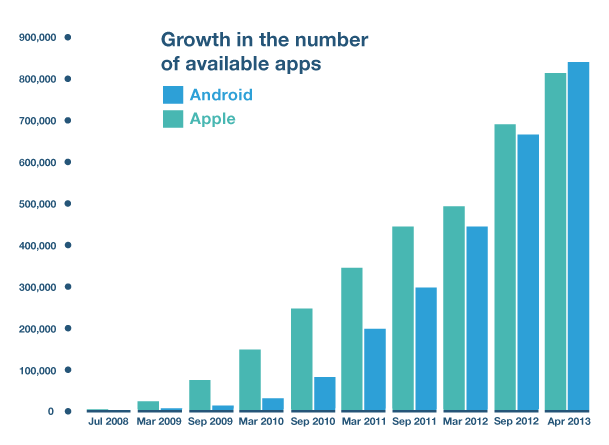
\includegraphics[width=13cm]{figures/app-bar-chart-3.png}
  \caption{Comparison of growth in number of available apps in App Store and Play Store. Source: http://www.appdomains.com/app-promotion/app-market-overview/}
  \label{fig:app-bar-chart-3}
\end{figure}

In the last four years, user contributed libraries for ruby programming language in http://rubygems.org have increased from 10,000 to more than 90,000 as the ruby language has gathered popularity \cite{modulecounts}. More recent examples would include Docker and Atom.io. Docker is an open-source project that automates the deployment of applications inside software containers. To promote more developer engagement, docker introduced Docker hub \cite{dockerhub}\cite{wiki:Docker_Software} where people can openly share their docker images. Similarly Atom.io calls themselves ``A hackable text editor for the 21st Century''. It also contains a repository for developers to contribute packages and themes \cite{atomiorepo}\cite{wiki:Atom_TextEditor}. Package contributions for both softwares have increased in the past few months.

The benefits of an app store can apply equally to Ubiquitous Computing platforms. \cite{dixon2010home} describe HomeOS and HomeStore. HomeOS is an operating system for managing different smart devices to create smart environment inside a home. Software developers can build applications and share them online in HomeStore, which is an app store for HomeOS similar to Apple's App Store for iOS. HomeStore recommends users with different software they can run inside their house. It also recommends the user about missing smart devices necessary to run certain applications. HomeStore also performs basic quality checks and supports ratings and reviews to help identify harmful or badly engineered applications.

Pahl recently completed his Ph.D. thesis on \emph{Distributed Smart Space Orchestration System (DS2OS)} \cite{pahl2014distributed}. He describes DS2OS as a platform that allows orchestration of smart environments. It includes a Software Development Kit (SDK) for developers to create different types of applications for smart spaces. It provides a runtime environment to run the software in distributed environment. DS2OS also consists of an app store named S2Store. Like with HomeStore for HomeOS and App Store for iOS, S2Store is a marketplace for smart space applications.

\section{Objective}

\cite{pahl2014distributed} list the two major challenges in Ubiquitous Computing platform which an app store can help overcome and explains how. The challenges being:

\begin{enumerate}
  \item Smart spaces have huge diversity of smart devices.
  \item Smart spaces have diversity of orchestration scenarios.
\end{enumerate}

\emph{Diversity of smart devices} means the existince of a wide variety of devices in the market available from different vendors. For mobile devices, the available hardwares are bound to predefined specifications. Most mobile devices have standard sensors and standard hardware parts. Applications build for mobile devices have less incompatibility issues. In contrast, electronic hardwares have no widely accepted standards when it comes to features. For e.g., a table lamp could vary in working from another table lamp from different vendor in the brightness of the bulb, the size of the lamp, lamp made for wall versus for the table, if it allows dimming the lamp, etc. Integration of these devices into pervasive computing environments require special hardware drivers. It is unlikely that vendors provide hardwares drivers for their devices when there isn't any standard platform.

\emph{Diversity of orchestration scenarios} means that there exists many different ways to orchestrate a smart space. For e.g., it is highly like for two houses to have different room structure, different requirements for entertainment, different interest of the house owners, etc. The kinds of different applications that can be written for all the different scenarios are huge. It is desired that applications are written in small and modular fashion and can interoperate with each other. Larger complex functionality is achieved by reusing smaller modules together. Such system does not exist for smart spaces.

The DS2OS framework with S2Store solves these issues by allowing crowdsourced development. Crowdsourcing is the process of obtaining needed services, ideas, or content by soliciting contributions from a large group of people \cite{pahl2014distributed}. Crowdsourced software development means software developers contributing to S2Store on a global scale. In S2Store, there are different entities that can be contributed by the crowd as described in Section \ref{sec:ds2os}.

Crowdsourcing results in:

\begin{enumerate}
  \item Large number of contributions and
  \item Varying quality of contributions.
\end{enumerate}

It is desirable to have large number of contributions in online app store. But, varying quality of contributions caused by varying skill, knowledge and experience of developers has to be taken into consideration. Identification of quality contents in large crowdsourced platforms is a common problem. Online marketplaces e.g. eBay, Amazon, StackOverflow uses reputation systems that label whether a certain user or the item she wants to trade, is good or bad, trustworthy or fake. Reputation Systems are special features added to online marketplace to create trust among users and mark qualities of different items. \cite{Resnick2000} and \cite{farmer2010building} describe reputation systems in detail.

An app store for smart spaces has similar requirements to that of any existing app stores for mobile platforms for trading purposes. In addition, an app store for smart spaces needs to consolidate challenge of having diverse hardware devices and orchestration scenarios. A smart space app store does this by creating a platform that allows collaboration of developers and early adopters to create standards themselves in a crowdsourced manner.

It is believed that given the vastness of the challenge present in developing softwares for smart spaces, reputation mechanisms are key parts of the solutions. The objective of the thesis is to understand the role of different reputation mechanisms in an online app store for smart spaces and how they play significant part by converging user opinions into default standards.